\documentclass[10pt,a4paper]{article}
\usepackage[utf8]{inputenc}\usepackage[T1]{fontenc}\usepackage[brazil]{babel}
\usepackage{geometry,graphicx,amsmath,booktabs,microtype}
\geometry{margin=1.65cm}\setlength{\parindent}{0pt}\setlength{\parskip}{3pt}
\title{\vspace{-1em}\textbf{Estimação de movimento com sensores ruidosos}\\\large Projeto 3 — Filtro de Kalman}
\author{Portfólio de Inteligência Artificial 1}\date{}
\begin{document}\maketitle\vspace{-1em}
\textbf{Resumo.} Este projeto estima posição e velocidade de um componente mecânico usando medições de posição contaminadas por ruído. O filtro linear manual inclui covariância do erro e a forma de Joseph, além de uma análise de especificação incorreta de $R$.
\section{Problema e modelo}
O estado é $\mathbf{x}_k=[p_k,v_k]^T$, com passo $\Delta t=0,5$ s e dinâmica quase uniforme:
\[
\mathbf{x}_k=F\mathbf{x}_{k-1}+\mathbf{w}_k,\quad
F=\begin{bmatrix}1&\Delta t\\0&1\end{bmatrix},\quad
z_k=H\mathbf{x}_k+v_k,\ H=[1\ 0].
\]
O processo usa $Q=\mathrm{diag}(0,01;0,01)$ e a medição nominal usa $R=4$. A trajetória sintética tem posição inicial 0, velocidade 1,2 e perturbação gaussiana de processo.
\section{Algoritmo}
Predição: $\hat{x}_{k|k-1}=F\hat{x}_{k-1|k-1}$ e $P^-_k=FP_{k-1}F^T+Q$. Na atualização, $S=HP^-H^T+R$, $K=P^-H^TS^{-1}$ e $\hat{x}_k=\hat{x}^-+K(z-H\hat{x}^-)$. A covariância usa a forma de Joseph:
\[
P_k=(I-KH)P^-(I-KH)^T+KRK^T,
\]
que preserva simetria e positividade melhor sob arredondamento.
\section{Experimentos e resultados}
Com semente 23 e 120 amostras, o erro bruto de posição foi RMSE $1,954$ e MAE $1,544$; após filtragem, RMSE $1,176$ e MAE $0,973$. Portanto, o ganho foi obtido sem observar diretamente a velocidade.
\begin{figure}[h]\centering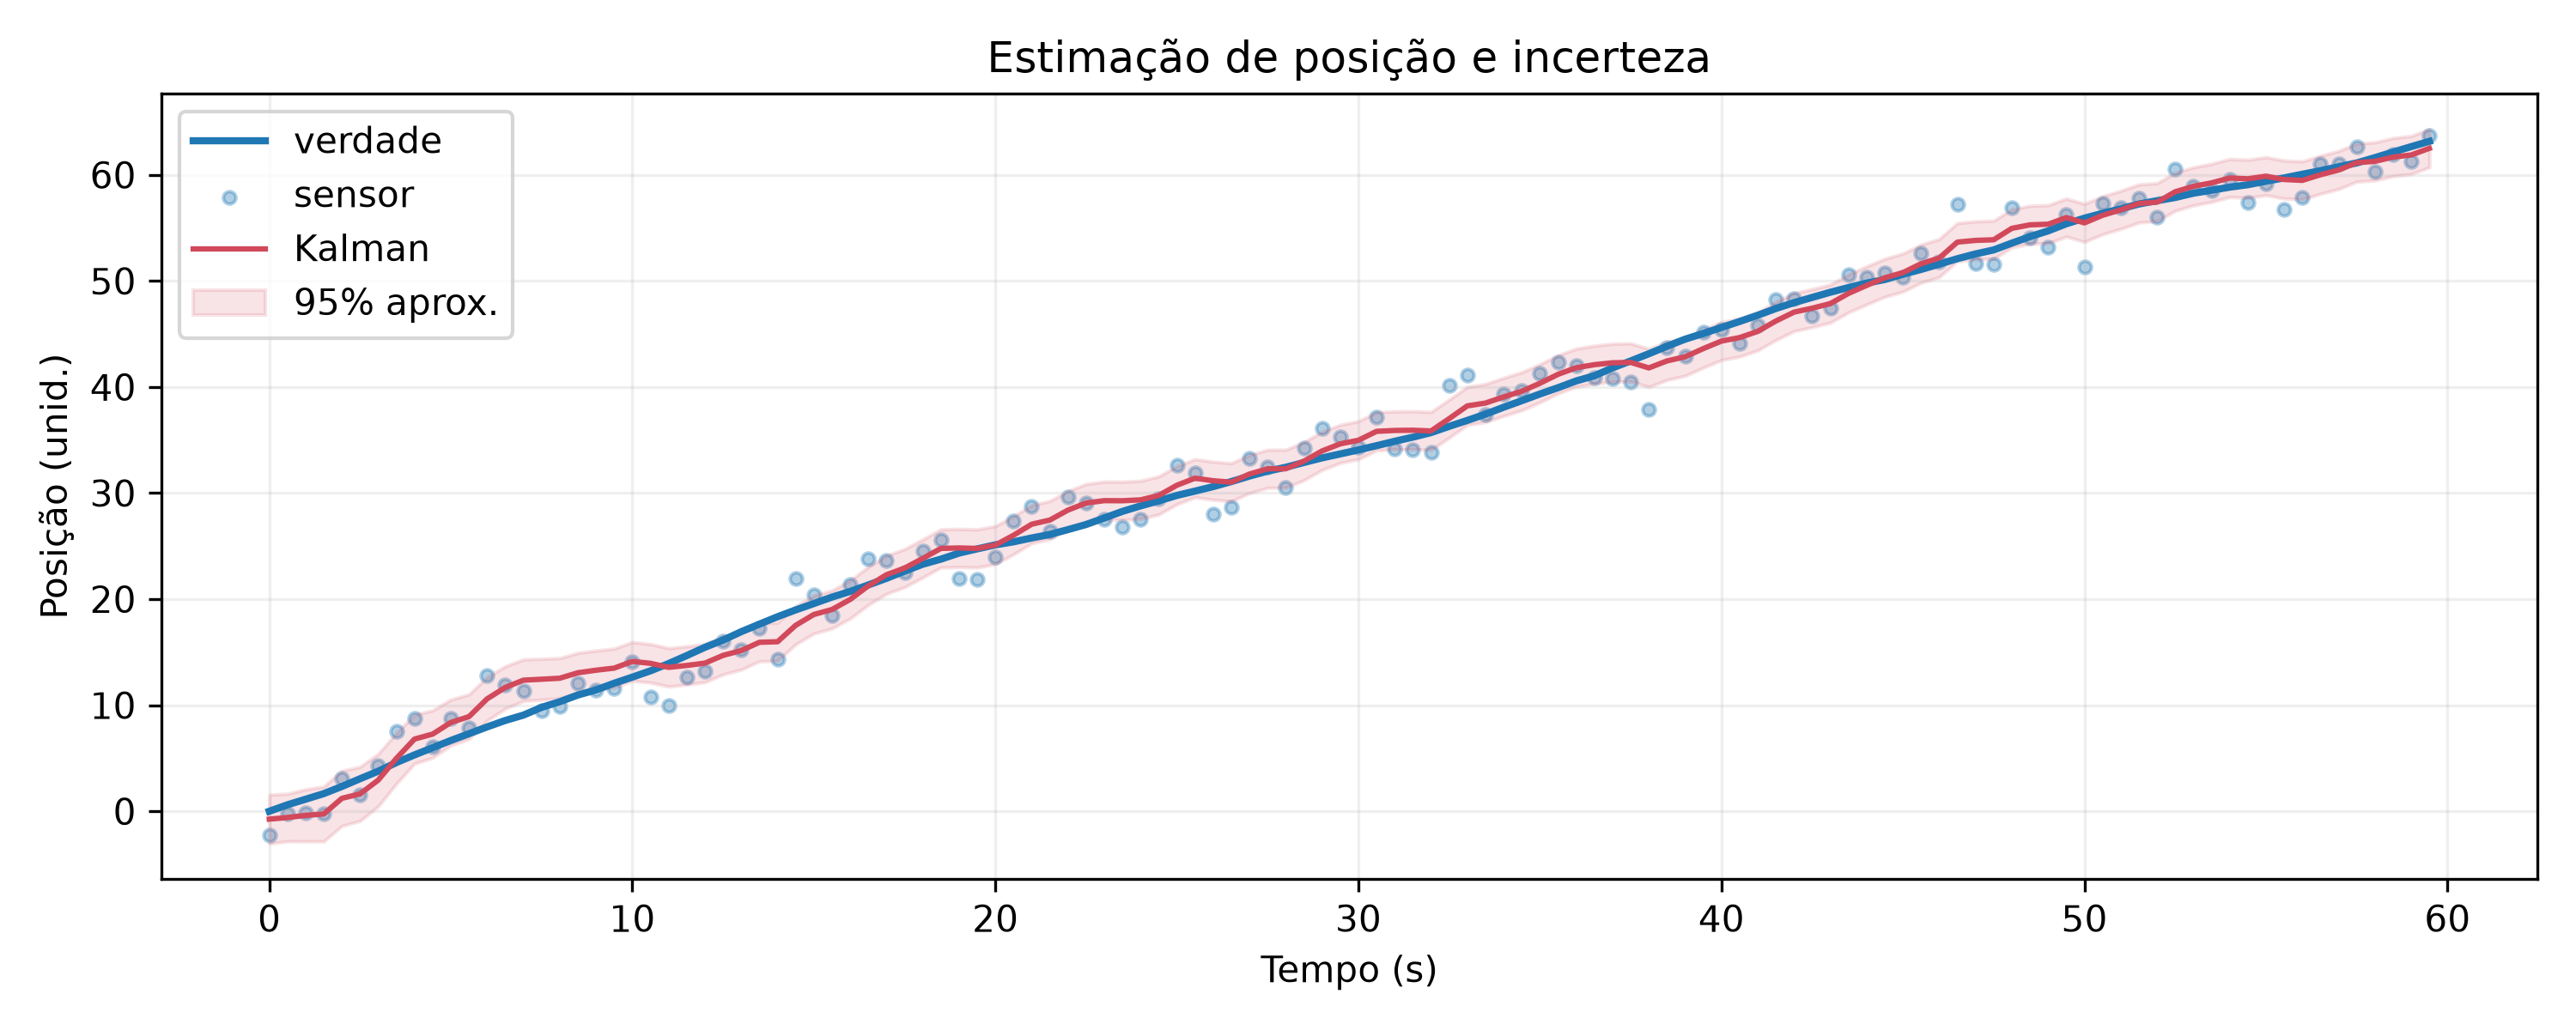
\includegraphics[width=.92\linewidth]{results/state_estimation.png}\caption{Trajetória, sensor, estimativa e intervalo aproximado de 95\%.}\end{figure}
\begin{figure}[h]\centering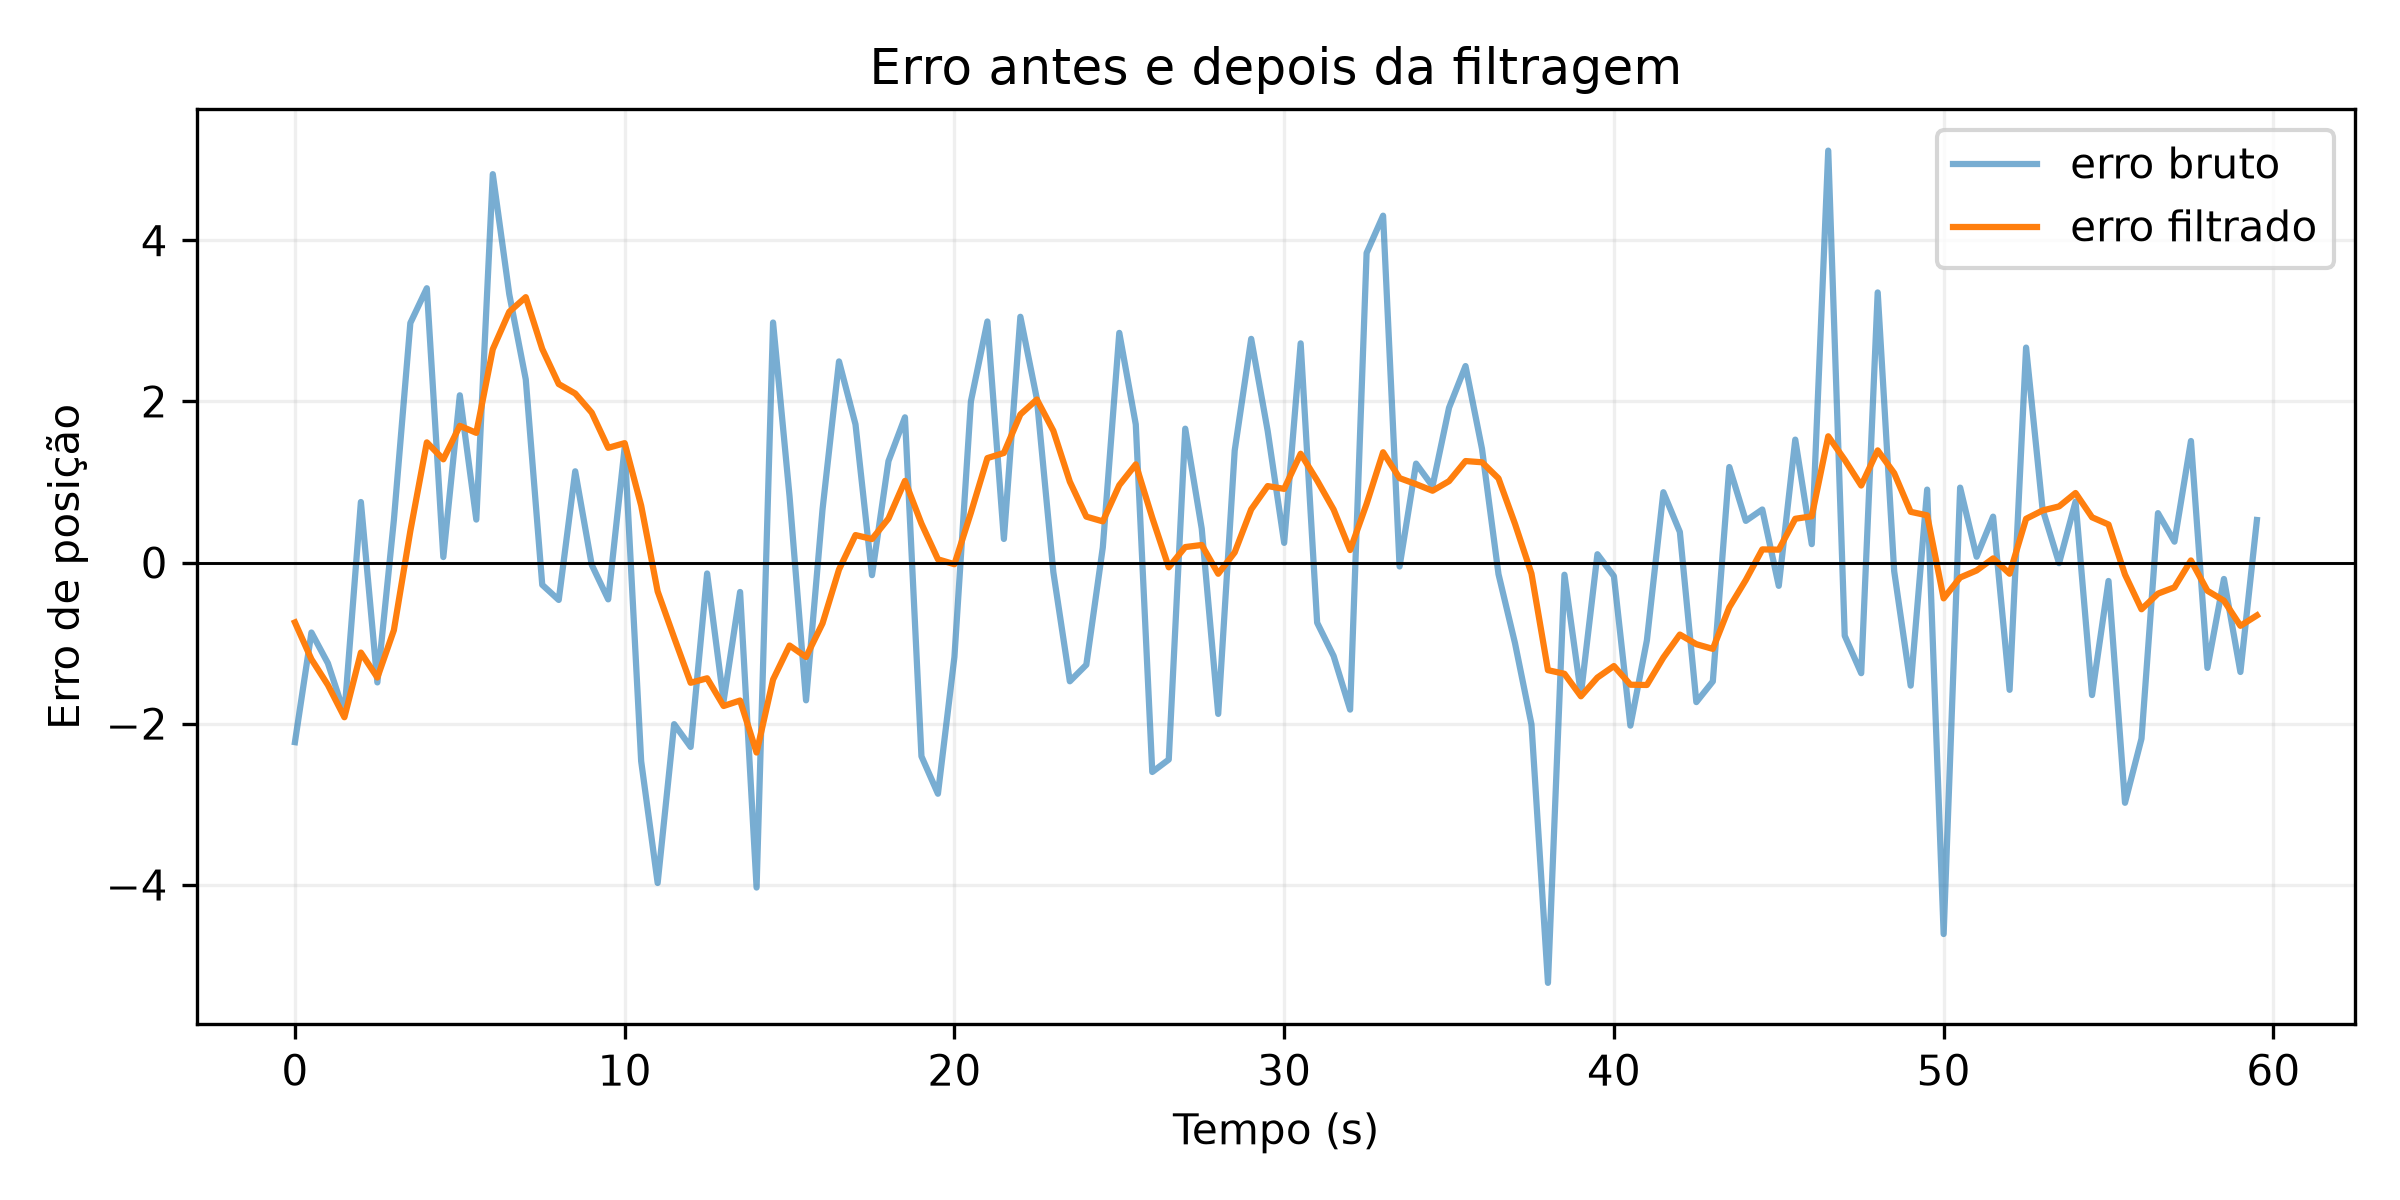
\includegraphics[width=.9\linewidth]{results/estimation_error.png}\caption{Erro de posição antes e depois do filtro.}\end{figure}
\begin{center}\small
\begin{tabular}{rrrrr}\toprule
R & 0,25 & 1 & 4 & 16\\\midrule
RMSE sensor & 0,489 & 0,977 & 1,954 & 3,909\\
RMSE Kalman & 0,379 & 0,689 & 1,176 & 1,902\\\bottomrule
\end{tabular}\end{center}
\begin{figure}[h]\centering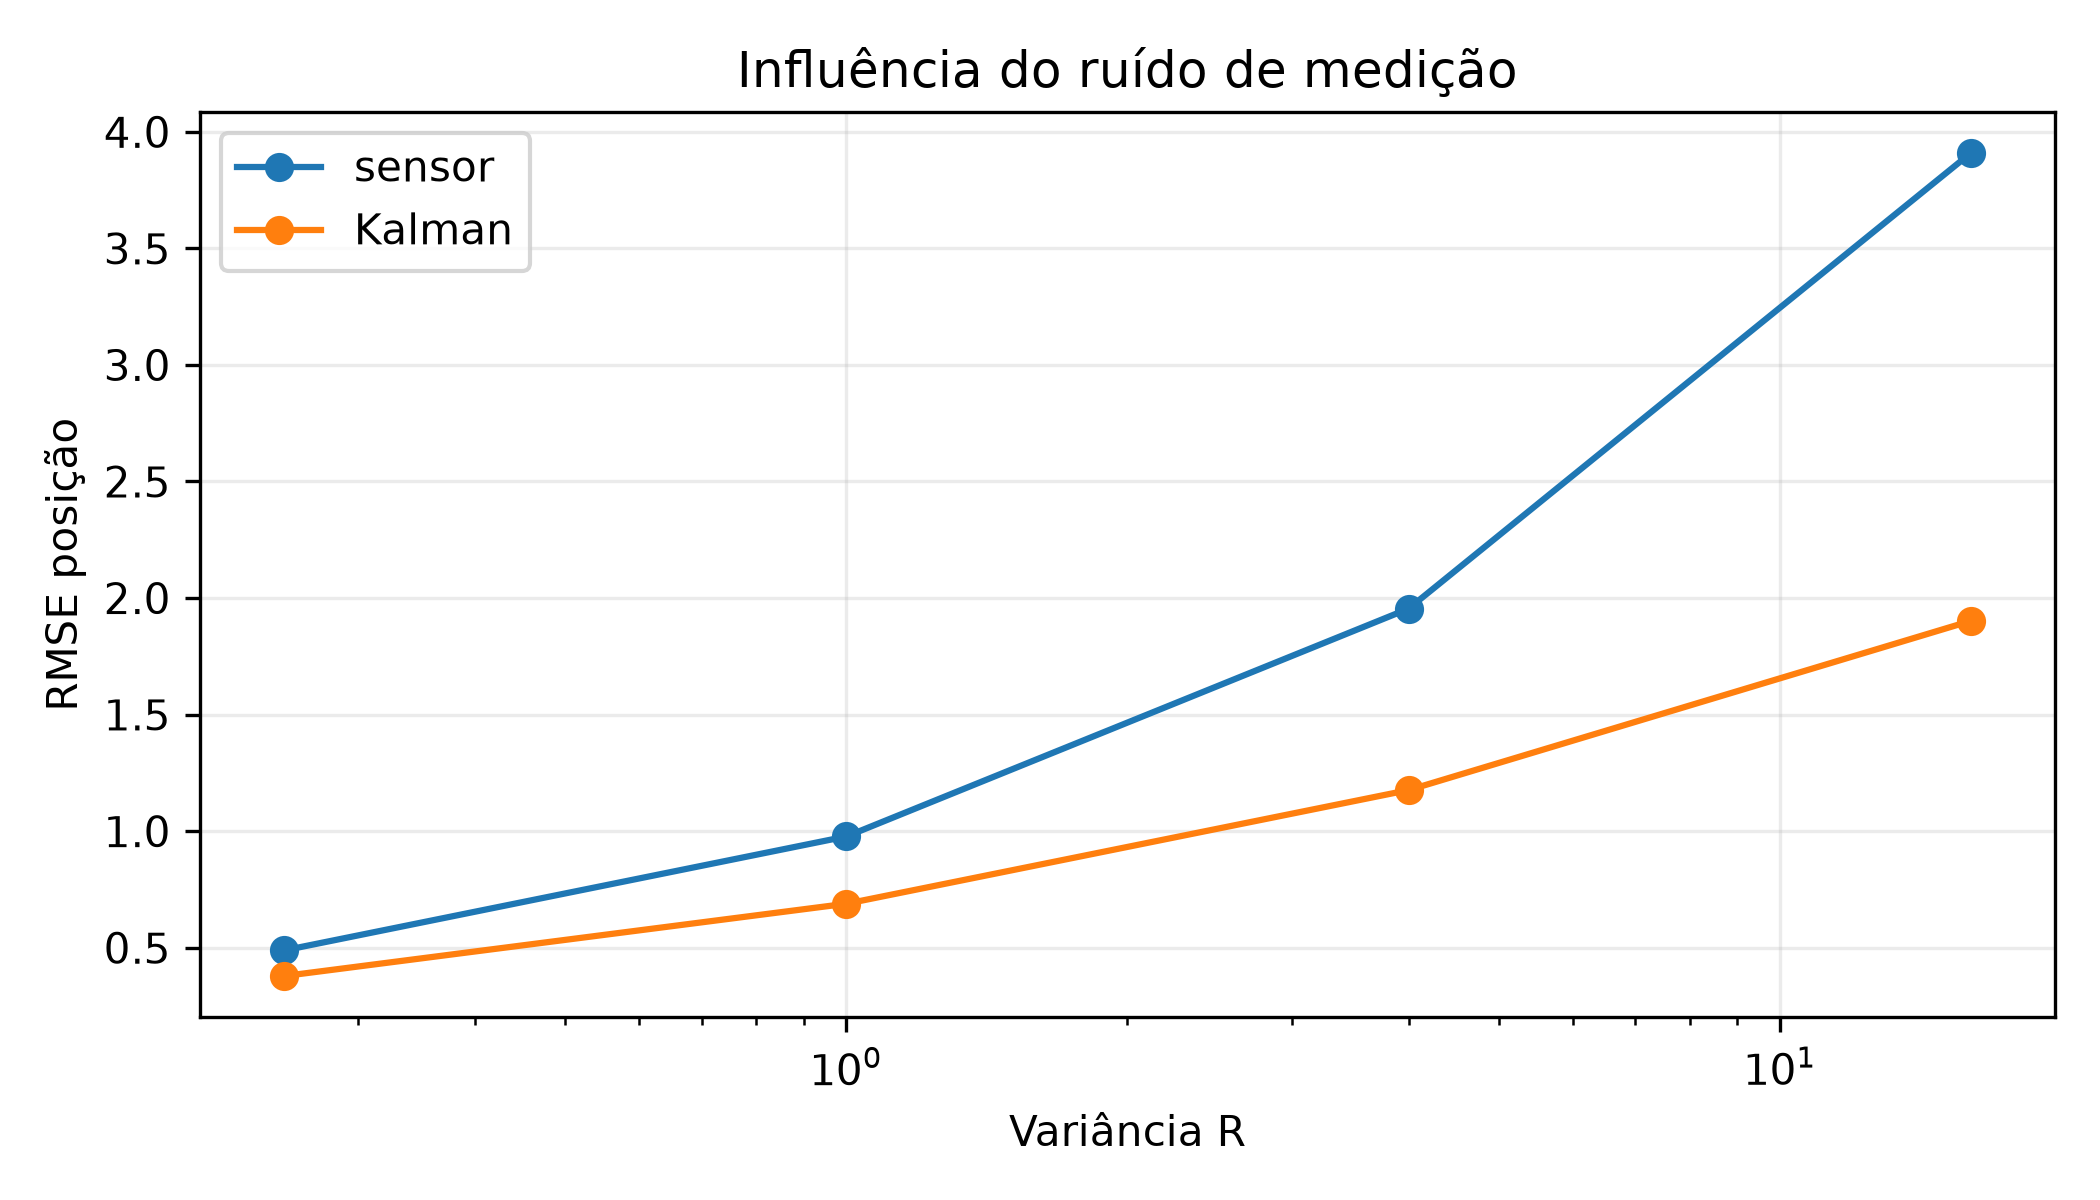
\includegraphics[width=.62\linewidth]{results/noise_comparison.png}\caption{Ruído maior aumenta ambos os erros, mas o filtro mantém vantagem.}\end{figure}
Quando o filtro assume $R=0,25$ embora o sensor tenha variância 4, o RMSE sobe para $1,386$: confiar excessivamente em medições ruins torna a estimativa mais instável.
\section{Conclusão}
O Kalman é adequado quando a dinâmica é aproximadamente linear e os ruídos têm covariâncias conhecidas. Ele suaviza sensores sem simplesmente aplicar média móvel, pois incorpora previsão física e incerteza. Modelos não lineares, ruídos não gaussianos e falhas de sensor exigem EKF/UKF, filtros robustos ou detecção de outliers. Referências: Kalman (1960); Simon (2006).
\end{document}
